\documentclass{report}

\usepackage[a4paper, left=2.5cm, right=2cm, top=1.5cm, bottom=2cm, includefoot=false, includehead=false]{geometry}
\usepackage[MeX]{polski}
\usepackage[utf8]{inputenc}
\usepackage{enumerate}
\usepackage{graphicx}

\makeatletter

\newcommand{\linia}{\rule{\linewidth}{0.4mm}}

\renewcommand{\maketitle}{\begin{titlepage}

    \vspace*{1cm}

    \begin{center}\small

    Politechnika Wrocławska\\

    Wydział Elektroniki W-4\\

    \end{center}

    \vspace{3cm}

    \noindent\linia

    \begin{center}

      \LARGE Projekt lokalne sieci komputerowe\\
      \normalsize\textsc{\@title}

         \end{center}

     \noindent\linia

    \vspace{0.5cm}

    \begin{flushright}

    \begin{minipage}{6cm}

    \textit{\small Autor:}\\

    \normalsize \textsc{\@author} \\

    \end{minipage}

    \vspace{5cm}

     {\small Prowadzący:}\\

         Dr hab. inż. Krzysztof Walkowiak

     \end{flushright}

    \vspace*{\stretch{6}}

    \begin{center}

    \@date

    \end{center}

  \end{titlepage}

}
\makeatother

\author{Mateusz Socha 181308 \\ Janusz Kuszczyński 184872 }

\title{}

\begin{document}

\maketitle
\tableofcontents

\chapter{Wstęp}
\paragraph{ZASTRZEŻENIE}
Firma, która jest zleceniodawcą tego projektu została wymyślona, wszelkie podobieństwa do prawdziwych firm są przypadkowe.
W miejscu podanym jako lokalizacja firmy obecnie znajduje się inne przedsiębiorstwo. Plany budynków użyte w projekcie są fikcyjne i opracowane tylko na 
potrzeby tego projektu.Ich zgodność z obowiązującym prawem buowlanym nie została w żaden sposób zweryfikowana.

\vspace{0,5cm}
Projekt instalacji sieciowej jest realizowany dla firmy ComputerBudy. Siedziba która jest jednocześnie przedmiotem tego projektu znajduje się
przy ulic Szwajcarska 22 w Wrocławiu.

\begin{figure}[h!]
  \centering
      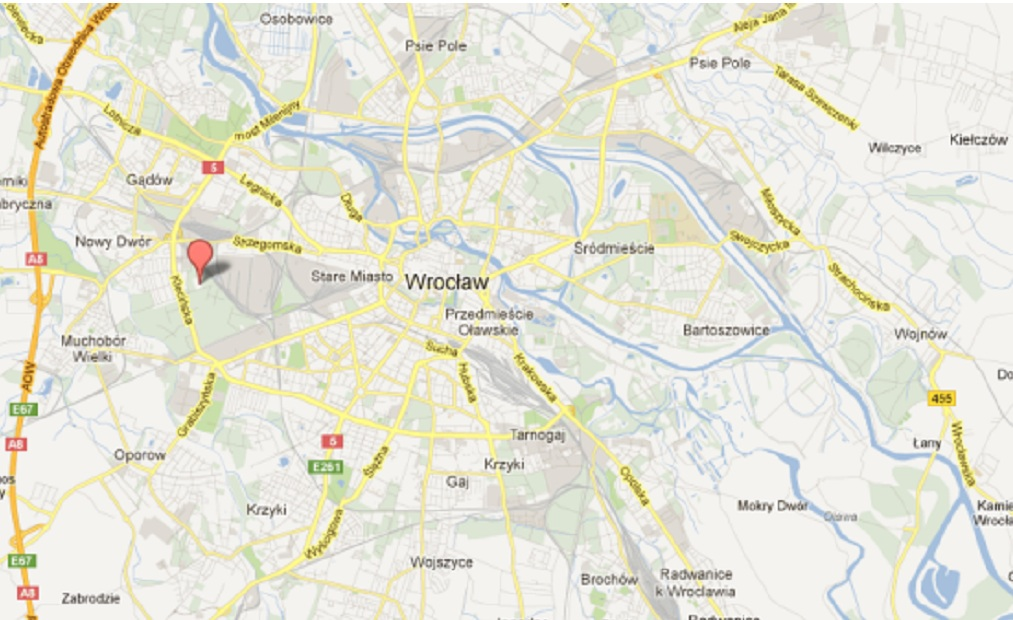
\includegraphics[width=0.8\textwidth]{./obrazki/adres_computerbudy.jpeg}
  \caption{Lokalizacja centrali firmy na mapie Wrocławia.}
\end{figure}

ComputerBudy jest firmą z działu IT. Zajmuje się ona zdalną pomocą przy problemach informatycznych. Zapewnia również zdalną administrację dla
skomplikowanych aplikacji na urządzeniach użytkownika. Jej oferta jest skierowana do osób prywatnych oraz małych i średnich firm, które
nie posiadają własnego działu IT.

Profil usług świadczonych powoduje, że brak połączenia z zewnętrzną siecią internet całkowicie paraliżuje całą firmę. 
Nawet awaria pojedyńczego stanowiska powoduje straty. Restrykcyjna polityka bezpieczeństwa firmy sprawia, że nawiązanie połączenia z klientem
może nastąpić tylko z sieci firmowej. Aby zwiększyć bezpieczeństwo każde stanowisko obsługujące klientów jest przyłączone do sieci
za pomocą stałego złącza ethernetowego. Obostrzenia te spowodowane są obawą przed podsłuchaniem poufnych informacji przez osoby niepowołane oraz
przejęciem kontroli nad komputerem klienta podszywając się pod pracownika firmy z innej lokacji.

ComputerBudy wynajmuje łącznie 4 piętra w dwóch bliźniaczych budynkach stojących obok siebie.W pierwszym dwa i w następnym budynku kolejne dwa.
Pozostałe piętra wynajmują inne firmy.

Celem naszego projektu jest stworzenie nowej instalacji teleinformatycznej na użytkowanych przez firmę piętrach w obu budynkach. Wnioskując z
profilu usług firmy priorytetowe znaczenie podczas projektowania należy nadać niezawodności. Drugim w kolejności czynnikiem jest oczywiście
szeroko pojęte bezpieczeństwo. Wskazane jest również zapewnienie łatwej możliwości rozbudowy sieci w tym budynku na kolejne piętra.
Oczywiście jako, że zleceniodawca jest firmą prywatną należy zminimalizować koszty całego przedsięwzięcia.

Do stworzenia projektu instalacji teleinformatycznej zostaną użyte szczegółowe plany budynków udostępnione przez zleceniodawcę.
Wymagania użytkowników zostaną opracowane na podstawie danych przekazanych przez administratora IT firmy oraz poprzez konsultację
z samymi pracownikami. Przepustowości łącz w nowej instalacji zostaną oszacowane na podstawie danych z obecnie istniejącej sieci komputerowej.

\chapter{Inwentaryzacja sprzętu i infrastruktury dostępnej w przedsiębiorstwie}
\chapter{Analiza potrzeb użytkowników – wymagania zamawiającego}
\chapter{Założenia projektowe}
\chapter{Projekt sieci}
\section{Projekt logiczny sieci wraz z opisem koncepcji rozwiązania}
\section{Konfiguracja adresacji IP}
\section{Projekt okablowania}
\section{Projekt podłączenia do Internetu}
\section{Analiza bezpieczeństwa i niezawodności sieci}
\section{Kosztorys urządzeń}

%Otoczenie tabelki
%\begin{table}
 % \caption{Geograficzne rozmieszczenie odziałów firmy.}
 %\includegraphics[width=0.9\textwidth]{./obrazki/topologia.jpeg}
%\end{table}

%\begin{figure}[h!]
 % \centering
 %     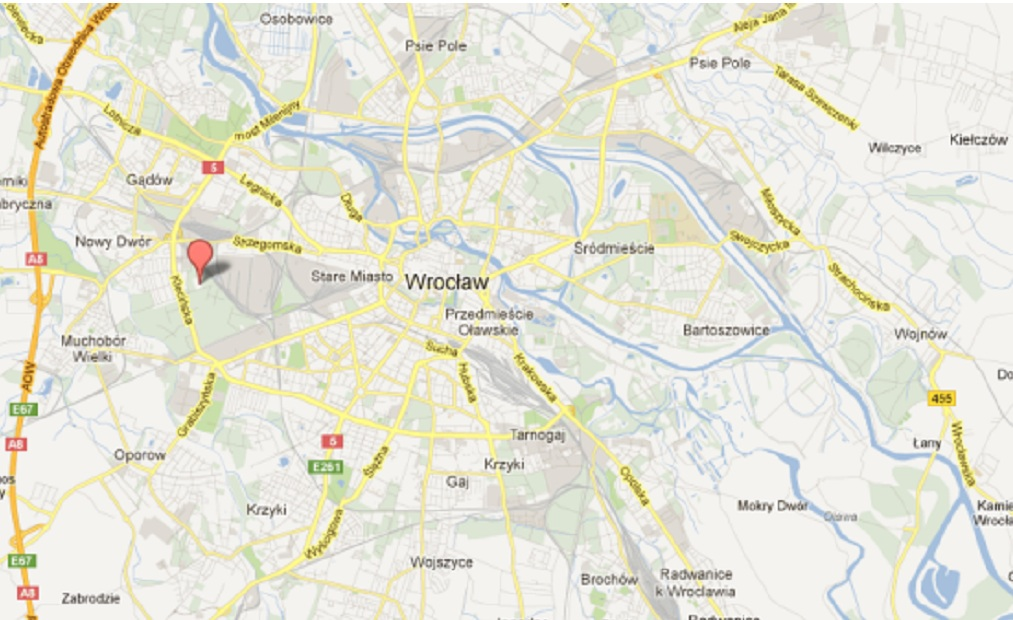
\includegraphics[width=0.9\textwidth]{./obrazki/adres_computerbudy.jpeg}
%  \caption{Geograficzne rozmieszczenie odziałów firmy.}
%\end{figure}

\chapter*{notatki}

literówki done

\end{document}
